\section{Konzept}
\subsection{Umfrage}
Im Rahmen der Projektvorbereitung soll auch eine Umfrage unter potenziellen Kunden erfolgen. So sollen möglichst früh in der Entwicklung Wünsche und die Sicht der Kunden auf ein Produkt oder ein Problem eingeholt werden. Hierbei handelt es sich um den sogenannten Customer Insight, welcher uns neue Perspektiven eröffnen soll. Damit soll verhindert werden, dass wir in unseren Ideen möglicherweise etwas ganz Entscheidendes vergessen, was aber aus der Sicht der Kunden besonders wichtig ist. Es sollen außerdem auch möglichst viele verschiedene Anforderungen der einzelnen Personen zu erhalten. Dafür haben wir eine Umfrage mit insgesamt 19 Fragen entwickelt. Am Ende konnten wir immerhin 44 Teilnehmende aufweisen.

Zuerst kamen ein paar Fragen zum Fahrzeug der Teilnehmer, z.B. von welcher Marke und wie alt es ist. Im zweiten Abschnitt stellten wir einige Frage zur Sicherheit der Fahrzeuge der Teilnehmer, z.B. wie sie gegen Diebstahl geschützt sind und ob schonmal etwas gestohlen wurde. Als nächstes folgten Fragen, mit denen wir direkte Bedürfnisse und Anforderungen für unser Produkt gewinnen wollten, unter anderem wurde gefragt, was ihn/sie an aktuell zu erwerbenden Autoalarmsystemen stört und wieviel er/sie maximal für ein solches System ausgeben würde. Zum Abschluss wurden noch ein paar persönliche Informationen für mögliche statistische Zusammenhänge abgefragt, wie Geschlecht, Alter und Beschäftigungsverhältnis.
Konkret wurden die folgenden Fragen gestellt:

\begin{itemize}
	\item Von welcher Marke ist dein Auto?
	\item Zu welcher Fahrzeugklasse gehört dein Auto?
	\item Welches Baujahr ist dein Auto?
	\item Wie teuer war dein Auto ungefähr und wieviel ist es jetzt noch wert?
	\item Wie wichtig ist dir dein Auto? (Emotionale Bindung usw.)
	\item Wie ist dein Auto gegen Einbruch und Diebstahl geschützt?
	\item Wie zufrieden bist du mit deiner Sicherheitslösung?
	\item Wurde dir bereits ein Auto geklaut oder es versucht?
	\item Wurde schon einmal in dein Auto eingebrochen oder es versucht?
	\item Wenn ja, was wurde geklaut?
	\item Wie ist dein Auto versichert?
	\item Wo parkst du dein Auto normalerweise?
	\item Um was hast du Angst, wenn dein Auto unbeaufsichtigt ist?
	\item Was stört dich an bisher käuflich erwerblichen Alarmsystemen für Autos bzw. was würdest du an diesen ändern?
	\item Wie viel würdest du für ein neues Alarmsystem für dein Auto ausgeben?
	\item Du bist... (männlich, weiblich, divers)
	\item Wie alt bist du?
	\item Wie ist dein derzeitiges Beschäftigungsverhältnis?
	\item Wie hoch ist dein monatliches Nettoeinkommen?
\end{itemize}
Die Umfrage wurde mit Hilfe von Google Forms realisiert und noch unter folgendem Link abrufbar: \href{https://forms.gle/qNTWM4qkF7ykG4tt9}Umfrage
\subsection{Persona} Moni

\subsection{Konzept} 
Nachdem wir also mit Hilfe der Umfrage und der Persona schon einen groben Eindruck bekommen haben, auf welche Zielgruppe unser Produkt passen könnte und welche Eigenschaften und Funktionen es erfüllen soll, erstellten wir ein erstes, grobes Konzept. Dieses Konzept beinhaltet alle wesentlichen Komponenten unseres Produkts und ist in der folgenden Abbildung schematisch dargestellt.
\begin{figure} [H]
	\begin{center}
		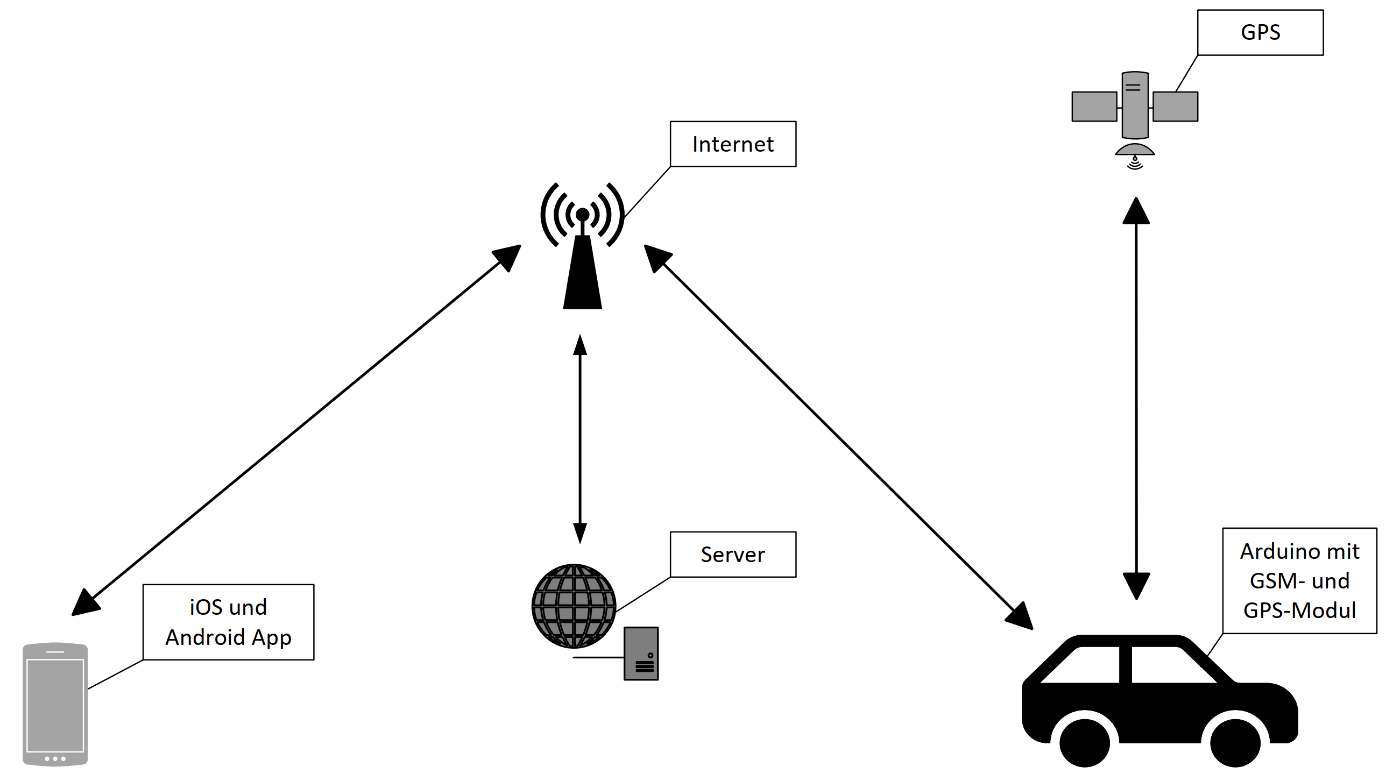
\includegraphics[width=1\textwidth]{Bilder/Konzept_Konzept.png}
		\caption{Systemkonzept}
		\label{konzept}
	\end{center}
\end{figure}
Im Fahrzeug wollen wir einen Arduino Uno zusammen mit einem passenden GSM- und GPS-Modul platzieren. Dieser ermittelt in bestimmten Zeitintervallen die aktuelle Position des Fahrzeugs und schickt die Koordinaten über die GSM-Verbindung an unseren Webserver. Dieser verarbeitet diese Daten und stellt sie anschließend so bereit, dass die Apps beider Betriebssysteme die aktuellen Koordinaten abfragen können.
